\documentclass[11pt,twoside,a4paper,BCOR8.25mm,DIV10,headsepline,footsepline,]{scrbook}
%------------------------------------------------------------------------------
%- PAKETE
%------------------------------------------------------------------------------
	%DIN A4
		\usepackage{a4}   
	%Ränder
		\usepackage[lmargin=2.5cm , rmargin=2.5cm]{geometry}

	%Fancy headers
		\usepackage{fancyhdr}
	
	%Sprache einstellen (Inhaltsverzeichnis, ...)
		\usepackage[english,ngerman]{babel} %american,italian,german
	
	%Euro Zeichen
		\usepackage{eurosym}	
		
		\usepackage[bookmarks=true,
					bookmarksopen=true,
   					% Lesezeichen ausgeklappt
					bookmarksnumbered=true,
					colorlinks=false,
				   	%Einf�rbung von Links
					linkcolor=black
					% Linkfarbe: schwarz					
					]
				    % Anzeige der Kapitelzahlen am Anfang der Namen der Lesezeichen
				   {hyperref}
		
	% Vereinfachtes Eingeben von Leerschl�gen hinter Shortcut-Commands
	% Beispiel: \newcommand{\DNA}{desoxyribose nucleid acid\xspace}
		\usepackage{xspace}
	
	%Sortierte Literaturverweise
		\usepackage{cite}
	
	%Grafiken
		\usepackage{float} %Float-Handling mit Schalter H (gleiche Position wie im Skript)
		\usepackage{floatflt}
		%\usepackage{flafter} %Verhindert Figuren vor ihrer ersten Referenz
		\usepackage{placeins} %Barriere f�r Float-Umgebungen erzeugen mit \FloatBarrier
	
	%Verbessertes Beschriften mir div. Optionen
		\usepackage[format=plain,labelsep=colon,labelfont=bf,textfont=it]{caption}
	
	%Zusaetzliche Symbole und Schriften (ams: american mathematical soc)
		\usepackage{amssymb}
		\usepackage{amsmath}
		%\usepackage{amstext}
		%\usepackage{amsfonts}
		%\usepackage{amsbsy}
		%\usepackage{amscd}
		%\usepackage{latexsym}

	%Text Companion fonts which provide many text symbols (such as baht, bullet, copyright, musicalnote, onequarter, section, and yen) in the TS1 encoding.
		\usepackage{textcomp}
	
	%Drehen von Text, Tabellen, Seiten
		%\usepackage{rotating}
	
	%including graphics files, rotating parts of a page, and scaling parts of a page
		\usepackage{graphicx}
	
	%Nice drawing package
		%\usepackage{tikz}               
	
	%besserer eps import: \eps import ERSETZEN durch \epsfig
		\usepackage{epsf}
	
	%Farbunterst�tzung (ausserhalb der Bilder)
		\usepackage{color}
	
	%Postcript einbinden, wobei Text ersetzt werden kann
		%\usepackage{psfrag}
	
	%F�r den Index
		\usepackage{makeidx}
		\makeindex %Muss vor begin{document}, sonst passiert nix
	
	%Erleichterungen f�rs Deutsche inkl Silbentrennung
		%\usepackage{german}
	
	%Ensure minimal spacing of table cells (http://www.ctan.org/tex-archive/help/Catalogue/entries/cellspace.html)
		\usepackage{cellspace}
	
	%Direkte Eingabe von Umlauten mit Angabe von Schriftsatz
	%in Kombination mit 'german' sind jetzt � direkt erlaubt!
		\usepackage[utf8]{inputenc}
	
	%Source code Listings 
		\usepackage{listings}
	
	%Darstellung von Algorithmen
		\usepackage{algorithm}
		\usepackage{algorithmic}
	
	%Subfigures
		\usepackage{subfigure}

%-- Fieser Hack f�r Subfigures (braucht man, um lstlistings im Subfigures zu nutzen)
\newbox\subfigbox
\makeatletter
\newenvironment{subfloat}
{\def\caption##1{\gdef\subcapsave{\relax##1}}%
\let\subcapsave\@empty
\setbox\subfigbox\hbox
\bgroup}
{\egroup
\subfigure[\subcapsave]{\box\subfigbox}}
\makeatother
	
	%Automatically adds the bibliography and/or the index and/or the contents, etc., to the Table of Contents listing.
		%\usepackage[nottoc]{tocbibind} %,notlot,notlof
	
	%St Mary Road symbols for theoretical computer science.
		%\usepackage{stmaryrd}
	
	%URL Darstellung
		\usepackage{url}


	%PDF und Standard Latex Unterscheidung
		\usepackage{ifpdf} 

	%Fancy verbose environments
		\usepackage{fancyvrb}	

	%Abk�rzungsverzeichnis
		\usepackage{nomencl}
		  \let\abbrev\nomenclature
		  \renewcommand{\nomname}{Abk�rzungsverzeichnis}
		  \setlength{\nomlabelwidth}{.25\hsize}
		  \renewcommand{\nomlabel}[1]{#1 \dotfill}
		  \setlength{\nomitemsep}{-\parsep}
		  \makenomenclature

	  \newcommand{\abk}[2]{#1\abbrev{#1}{#2}}
				
	%With \usepackage{ulem}, you have the following new commands:
		%    * \uline{important} underlined text
		%    * \uuline{urgent} double-underlined text
		%    * \uwave{boat} wavy underline
		%    * \sout{wrong} line drawn through word
		%    * \xout{removed} marked over with //////.
		%    * {\em phasized\/} and \emph{asized} In LaTeX, by default, these are underlined; use \normalem or [normalem] to restore italics
		%    * \useunder{\uwave}{\bfseries}{\textbf} use wavy underline in place of bold face 
		%Note that this package changes \em and \emph to be underline. To change this behavior back to normal, use the \normalem command, for example
		%\usepackage{ulem}
		%\normalem
		%\usepackage[normalem]{ulem}

	  %\newcommand{\markup}[1]{\uline{#1}}	

	% package to customize the three basic lists (enumerate, itemize and description) 
	% by means of a set of parameters, and to clone them to define new "logical" lists.
		\usepackage{enumitem}
		\setitemize{enumsep=-3pt}
		\setitemize{itemsep=-3pt}

	%Definitionen
		\usepackage{theorem}
		\newcounter{theorem}
		\newtheorem{definition}[theorem]{Definition}

	%Zitate
		\newcounter{quotectr}
		\newtheorem{myquote}[quotectr]{Zitat}

%------------------------------------------------------------------------------
%- Layout
%------------------------------------------------------------------------------

	%Tiefe des Inhaltsverzeichnisses und der Nummerierung der Kapitel
		\setcounter{secnumdepth}{2}
		\setcounter{tocdepth}{2}

	%Call this after each chapter to avoid headlines on empty pages
		\newcommand{\chapterfin}{\clearpage{\pagestyle{empty}\cleardoublepage}}
		\newcommand{\sectionfin}{\clearpage{\pagestyle{empty}\cleardoublepage}}

	% Listings schoen machen 
		\renewcommand*\ttdefault{txtt}
	
		\lstset{%
		  breaklines=true,
		  basicstyle=\ttfamily\footnotesize,%
		  moredelim=[is][\fontseries{lt}\bfseries]{|}{|},%
		  captionpos=b,%
		  numbers=left,%
		  tabsize=1,%
		  numberstyle=\tiny,%
		  numbersep=6pt,%
		  frame=lr,%
		  framesep=0pt,%
		  framexleftmargin=5pt,%
		  framextopmargin=0pt,%
		  framexbottommargin=0pt,%
		  xleftmargin=15pt,%
		  xrightmargin=15pt,%
			abovecaptionskip=0pt,%
			belowcaptionskip=-0pt,%
		}	
		
		\lstdefinelanguage{XMLSchema}
			{morekeywords={schema,element,annotation,appinfo,complexType,simpleType,choice,all,sequence},		
			sensitive=true,
%			morecomment=[l]{//},
%			morecomment=[s]{/*}{*/},
			morestring=[b]",
		}
		
		\lstdefinelanguage{ASN1}
			{morekeywords={},		
			sensitive=true,
%			morecomment=[l]{//},
%			morecomment=[s]{/*}{*/},
			morestring=[b]",
		}
		
	
	% Font
	%
	%	Danach muss man die Standardschriftart setzen mit dem Befehl \fontfamily{abr}\selectfont, 
	% der f�r das gesamte restliche Dokument gilt, oder mit {\fontfamily{abr}\selectfont Some Text} 
	% um nur den eingeklammerten Bereich zu betreffen. abr ist die Abk�rzung f�r die Schriftart. Die 
	% h�ufigsten sind ptm (Times), phv (Helvetica), pcr (Courier), pbk (Bookman), pag (Avant Garde), 
	% ppl (Palatino), bch (Charter), pnc (New Century Schoolbook), pzc (Zapf Chancery), put (Utopia ).

	% Sch�nerer tt font:
		%\renewcommand{\ttdefault}{pcr}
		%\selectfont
	
	% Times
		%\usepackage{times}
		
	%	Helvetica
			%\usepackage{helvet}
			%\renewcommand{\familydefault}{\sfdefault}
			%\renewcommand{\familydefault}{phv}
			%\fontfamily{abr}\selectfont
			
	%	Courier
			%\usepackage{courier} \raggedright
			%\renewcommand{\familydefault}{\ttdefault}
	
	% Absatzformatierungen:
	% Keeps the distance between paragraphs constant
		\setlength{\parskip}{1.5ex plus 0.0ex minus 0.0ex}
		\setlength{\parindent}{0pt}
	
	% Modify the placement of figures: from faq source: You can adjust the cut-off value if you like, 
	% but it makes no sense to go higher than .95 (LaTeX's default value is only .5). Also, the first 
	% 3 values should be equal, and the last should be 1 - \floatpagefraction.  Otherwise, you are 
	% likely to get floats flushed to the end. 
		\renewcommand{\floatpagefraction}{0.9}
		\renewcommand{\topfraction}{0.9}
		\renewcommand{\bottomfraction}{0.9}
		\renewcommand{\textfraction}{0.1}
		\renewcommand{\textfloatsep}{5mm}
	
	% Zeilenabstand
		\renewcommand{\baselinestretch}{1.25}

	% Fancyheaders 	
		\fancyhf{} % Delete all fields
		%\fancyhead[EL,OR]{\thepage}
		\fancyhead[EL]{\nouppercase{\leftmark}}
		\fancyhead[OR]{\nouppercase{\rightmark}}
		\fancyfoot[EL,OR]{\thepage}	
		
	% Itemize look and feel
		\renewcommand{\labelitemi}{\rule[+0.9mm]{2.7pt}{2.7pt}}
		\renewcommand{\labelitemii}{--}
		%\renewcommand{\labelitemiii}{}
		%\renewcommand{\labelitemiv}{\#}	

	% Floats richtig benennen:
		%\floatname{algorithm}{Algorithm}
		%\renewcommand{\listalgorithmname}{Algorithmen}
		
%------------------------------------------------------------------------------
%- Textbausteine
%------------------------------------------------------------------------------

	%Helpers
		\newcommand{\todo}[1]				{{\em [#1]}\marginpar{{\bf [!!!]}} }
		
		\newcommand{\eigenname}[1]	{{\em #1}}
		
	%Deutsch
		\newcommand{\figref}[1]{Abbildung~\ref{fig:#1}}
		\newcommand{\tabref}[1]{Tabelle~\ref{tab:#1}}
		\newcommand{\equref}[1]{Gleichung~\ref{equ:#1}}
		\newcommand{\chapref}[1]{Kapitel~\ref{cha:#1}}
		\newcommand{\appref}[1]{Anhang~\ref{cha:#1}}
		\newcommand{\secref}[1]{Abschnitt~\ref{sec:#1}}
		\newcommand{\lstref}[1]{Listing~\ref{lst:#1}}
		\newcommand{\algref}[1]{Algorithmus~\ref{alg:#1}}
		\newcommand{\ssecref}[1]{Unterabschnitt~\ref{ssec:#1}}
		\newcommand{\quoteref}[1]{Zitat~\ref{quote:#1}}

	%Englisch	
		%\newcommand{\figref}[1]		{Figure~\ref{fig:#1}}
		%\newcommand{\tabref}[1]		{Table~\ref{tab:#1}}
		%\newcommand{\equref}[1]		{Equation~\ref{equ:#1}}
		%\newcommand{\algref}[1]		{Algorithm~\ref{alg:#1}}
		%\newcommand{\defref}[1]		{Definition~\ref{def:#1}}
		%\newcommand{\quoteref}[1]	{Quote~\ref{quote:#1}}
		
		%\newcommand{\chapref}[1]	{Chapter~\ref{cha:#1}}
		%\newcommand{\appref}[1]		{Appendix~\ref{cha:#1}}
		%\newcommand{\secref}[1]		{Section~\ref{sec:#1}}
		%\newcommand{\ssecref}[1]	{Section~\ref{ssec:#1}}
		%\newcommand{\sssecref}[1]	{Section~\ref{sssec:#1}}
		
	% REDEFINE UGLY STUFF
		\renewcommand{\leq}		{\leqslant}
		\renewcommand{\geq}		{\geqslant}
		\renewcommand{\epsilon}	{\varepsilon}
		\newcommand{\musec}		{$\mu sec$\xspace}
		\newcommand{\muW}		{$\mu W$\xspace}
		\newcommand{\plusminus}	{$\pm $\xspace}
	
%------------------------------------------------------------------------------
%- Worttrennung
%------------------------------------------------------------------------------
	
	%\hyphenation{Ge-samt-ozon}	
	\hyphenation{name-space}	
	\hyphenation{name-spaces}	
	\hyphenation{ge-samten}	
			
%------------------------------------------------------------------------------
%- Grafiken
%------------------------------------------------------------------------------

	\ifpdf
	  \DeclareGraphicsExtensions{.jpg,.pdf,.png}   % for pdftex driver
	\else
	  \DeclareGraphicsExtensions{.eps}             % for dvips driver
	\fi
	
	% Vereinfacht die Einbettung von Grafiken
	% Beispiel: \myfig[5cm]{psdatei}{�bersicht �ber das Gesamtsystem}
	\newcommand{\myfig}[3][\columnwidth]
	{
	 \begin{figure}[htbp]
		 \begin{center}
			 \includegraphics[width=#1]{img/#2}
			 \caption{#3}
			 \label{fig:#2}
		 \end{center}
	 \end{figure}
	}
	
	\newcommand{\myfigtwo}[4][\columnwidth]
	{
		 \begin{figure}[htbp]
				\begin{center}
				  \mbox
				  {
				    \subfigure[#2] 
				    { \includegraphics[width=.45\columnwidth]{img/#1-a} \label{fig:#1-a} } 
				    \quad
				    \subfigure[#3]
				    { \includegraphics[width=.45\columnwidth]{img/#1-b} \label{fig:#1-b} }
			    }
				  \caption{#4}
					\label{fig:#1}
				\end{center}
			\end{figure}
	}
	
	\newcommand{\myfigthree}[5][\columnwidth]
	{
		 \begin{figure}[htbp]
				\begin{center}
				  \mbox{
				    \subfigure[#2]
				    {
				    	\includegraphics[width=.3\columnwidth]{img/#1-a}
				    	\label{fig:#1-a}
				    } 
				    \subfigure[#3]
				    {
							\includegraphics[width=.3\columnwidth]{img/#1-b}
				    	\label{fig:#1-b}
				    }
				    \subfigure[#4]
				    {
							\includegraphics[width=.3\columnwidth]{img/#1-c}
				    	\label{fig:#1-c}
				    }
			    }	
				  \caption{#5}
					\label{fig:#1}
				\end{center}
			\end{figure}
	}
	
	\newcommand{\myfigfour}[6][\columnwidth]
	{
		 \begin{figure}[htbp]
				\begin{center}
				  \mbox
				  {
				    \subfigure[#2] 
				    { \includegraphics[width=.45\columnwidth]{img/#1-a} \label{fig:#1-a} } 
				    \quad
				    \subfigure[#3]
				    { \includegraphics[width=.45\columnwidth]{img/#1-b} \label{fig:#1-b} }
			    }
				  \mbox
				  {
				    \subfigure[#4] 
				    { \includegraphics[width=.45\columnwidth]{img/#1-c} \label{fig:#1-c} } 
				    \quad
				    \subfigure[#5]
				    { \includegraphics[width=.45\columnwidth]{img/#1-d} \label{fig:#1-d} }
			    }
			    
				  \caption{#6}
				\label{fig:#1}
				\end{center}
			\end{figure}
	}
	


%Um die Abkuerzungen zu ermoeglichen:
% 	makeindex.exe thesis.nlo -s nomencl.ist -o thesis.nls
%   als Postprocessor in Texniccenter einrichten

% Nette Hinweise zum LaTexen einer Diss: 
% - http://iacweb.ethz.ch/en/various/Mittelbau/disslatex.html
% - http://www.zib.de/pfetsch/Diss-Styles/
% - http://www2.informatik.hu-berlin.de/~nlohmann/arbeit/koma.html

% Hiermit kann man festlegen, dass immer nur ein bestimmter Teil übersetzt wird
%\includeonly{1-einleitung}
\definecolor{orange}{RGB}{255,204,102}
\begin{document}
\selectlanguage{english}
\frontmatter

%---------------------------------------------------------------------------
% Frontpage
%---------------------------------------------------------------------------
	%---------------------------------------------------------------------------
% Frontpage
%---------------------------------------------------------------------------

\begin{titlepage}

\author{Maximilian Mühlfeld}

\let\footnotesize\small
	\let\footnoterule\relax
	\null
	\vfil
	\vskip 30pt
	\begin{center}
		{\LARGE
		  {
\includegraphics[width=80mm]{Logo_Uni_Luebeck_300dpi.png}
			\\
			\vskip 15pt
			\Large Universität zu Lübeck}\\
			Institute for Robotics and Cognitive Systems \\[2cm]
			{\Large Master Thesis}\\ [1cm]
			An Approach to Solving Object Displacement Problems 
			\par}%
		\vskip 4em
		{\large \lineskip .75em
		\begin{tabular}[t]{c}
			{\Large written by}\\[.5em]
			{\Large Maximilian Mühlfeld (580070)}\\\\
			{\bf Supervisor:}\\[.5em]
			Prof. Dr.-Ing. Achim Schweikard
		\end{tabular}
		\par}%
		\vfill 
		{\large
			Lübeck, \today
			\par}%
	\end{center}
	\par
	% thanks
	\vfil
	\null
\end{titlepage}

%\cleardoublepage

% Erklaerung
\newpage
\vspace*{1cm}
\centerline{\bf Assertion}

\vspace*{1cm}
I assure that the following work is done independently with the use of only stated 
resources.

\vspace*{3cm}
Lübeck, \today 
\newpage

%\vspace*{3cm}
%L�beck, den \today 


%\vspace*{3cm}
%L�beck, den \today 


%\vspace*{3cm}
%L�beck, den \today 

\pagestyle{headings}

%\cleardoublepage

% Kurzfassung und Abstract
\centerline{\bf Abstract}



%
\vskip 2cm
%

%\centerline{\bf Abstract}
%\bigskip
%This thesis in short.

%\cleardoublepage
The scope of this thesis grasps the implementation and testing of algorithms to solve object displacement problems.\\
To achieve this, the search space is divided into multiple cells to reduce its size. Furthermore, instead of calculating the whole space at once, a local approach is used to only calculate the parts needed for the next search step. This needs a wide range of basic geometric and algebraic algorithms for object representation, collision detection and object translation as well as rotation.\\
On the resulting search space a simple and exchangable graph search algorithm is applied, which gives a path in the object space from the
start configuration to the desired target configuration.

%%
%\vskip 4cm
%%
%\centerline{\bf Abstract}
%
%
%
%%
%\vskip 2cm
%%
%
%%\centerline{\bf Abstract}
%%\bigskip
%%This thesis in short.
%
%%\cleardoublepage
%The scope of this thesis is the implementation and testing of algoritms to solve object displacement problems.\\
%To achieve this the search space is divided into multiple cells to reduce its size. Furthermore instead of calculating the whole space at once, a local approach is used to only calculate the parts needed for the next search step. This needs a wide range of basic geometric and algebraic algorithms for object representation, collision detection and object translation/rotation.\\
%On the resulting search space a simple and exchangable graph search algorithm is applied, which will give us a path in the object space from
%start configuration to the desired target configuration.

%---------------------------------------------------------------------------
% Inhaltsverzeichnis
%---------------------------------------------------------------------------
	\tableofcontents
	%\cleardoublepage

%---------------------------------------------------------------------------
% Der eigentliche Inhalt
%---------------------------------------------------------------------------
	\mainmatter
	\pagestyle{fancy}
	
	\chapter{Introduction}
\label{cha:Introduction}

\section{Motivation}
\label{sec:Motivation}
\subsection{Path planning in robotics}
In the field of robotics the path planning of an industrial robot can be programmed as a fixed list of movements to be executed. This has multiple drawbacks as for every change in the enviroment the robot needs to manually be reprogrammed.\\
But what if we equip this robot with a camera that detects the shape of objects in the robots enviroment. This would give us a set of objects at certain positions, a robot arm in a starting position and a target where the robots endeffector needs to work. If we would be able to solve this puzzle, we could direct the robot in a different way each time without the actual need to access its software.


\subsection{Geometric riddles in gaming}
Solving geometric riddles is an amazingly fun task for a human. This is the reason many games simply consists of such riddles ranking from easy to hard in difficulty. But even the easiest riddle for a human proposes a big challenge for a simple algorithm that searches trough the possible ways of solving it. Even more complicated is the generation of such riddles. Even for the human brain this task can be exceedingly stressful.\\
 Now, if there would be a possibility to check if such a riddle has a solution, there would be the option to generate them randomly and check for feasibility. This would cast off the necessity for the developers to manually create each riddle. Also the consumers, in this case the players, would have a endlessly stream of new and different riddles to solve.


\section{Idea}
\label{sec:Idea}
For simplification purposes we let our algorithms work on two dimensional object displacement problems. The following riddles shall provide simple examples of the problem:\\

\begin{figure}[h]\centering

\includegraphics[scale=0.1]{circleRiddle.png}
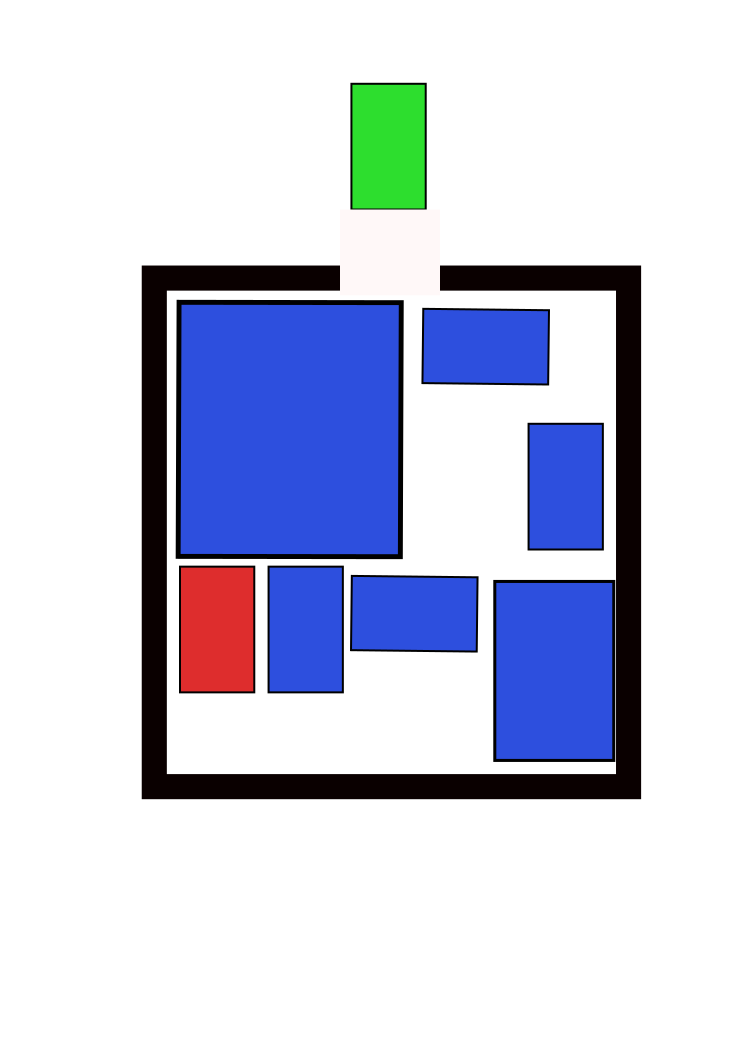
\includegraphics[scale=0.1]{boxRiddle.png}

\includegraphics[scale=0.1]{mixedRiddle.png}
\caption{riddle 1 with circles , riddle 2 with boxes , riddle 3 with 2 half-circles}
\end{figure}

The riddle is solved, if the red box matches the green one. Blue objects are movable and black ones are stationary. The stationary ones will be referred to as rims hereafter.\\
As a human the way to solve those is quite obvious. The first riddle is solved by rotating the blue objects, the second through translation. The third needs both ways to be solved.\\
If we want to solve this with an algorithm, we would need to consider each objects collsision with the other objects and the rim. Also we would need to find a way to express the current configuration consisting of position (x,y) and rotation ($\phi$) and the direction the main object needs to take. A first idea would be to 
\begin{enumerate}
\item Generate all valid configurations per object in regard to the stationary obstacles as a configuration space
\item Create one collision space per object for collision with every other object. 
\item Substract the collision space from the configuration space to get valid space in regard to all obstacles for one object.
\item Divide the space in cells and locate the valid ones.
\item Build a graph out of this starting position by adapting the space after each step.
\item Search in that graph to get a path from start to target point.
\end{enumerate}

The target point would then be a simple configuration vector holding each position of each object. A user defined distance function beetween start and target point in that space can then be used as heuristic in the graph search, e.g. $h(start,target) = || ( x_{start} -  x_{target} , y_{start} - y_{target} ) ||$ .


\section{State of the art}
\subsection{Pathplanning}
The correct answer to the question "Which algorithm is the best for finding the path from start to target" is not as easy as one might suspect. 
It depends on many factors including which structure one searches on ( e.g. graph, net, tree ), what knowledge there is about the current position ( e.g. distance to target ) and what result is needed ( shortest path, "good" path, existence of a path ).\\
For this work the focus is on an algorithm working on a graph with non-negativ edges, an absolute knowledge of the position of the target and the current in a two dimensional coordinate system and a need for a "good" path, not necessarily the shortest. Given these conditions, A$^\star$ is a valid choice. It is a widely used algorithm which calculates a "good" path, not a perfect one. How good the path is depends heavily on the heuristic used. In our case that would be a weighted sum of the distance traveled in steps plus the absolute distance to the target.\\
Another choice could be Dijkstra's algorithm \cite{ComputerScience} itself which is basically A$^\star$ with the heuristic set to constant zero. This would return the shortest path for all calculations. For the named applications from \ref{sec:Motivation} we need the algorithm to be fast, more than to be precise, thus A$^\star$ is the better choice.\\
It should be noted though that the algorithm for pathplanning is exchangable, as long as it is possible to create the graph while searching.

\subsection{Collision detection}
Collision detection in computer science has its home in simulations and computer games as it has in robotics. In this case the focus lies on the way computer games solve collision detection without looking into physical problems that would arise with it.\\
There are a number of ways this has been solved. In a case where there are not that many objects needed to check, pairwise checking is an option. Depending on how the objects are represented, they need to be checked for collision for every step taken. A way around this is to bound objects that lie in a certain proximity of each other together in spheres, where they are only checked in pairs if the spheres containing the objects collide.\\
Also there is a difference in checking if a collision happened, or if it is about to happen. The first option is easy to calculate, because all that is needed is the current position of the objects concerned. The second needs to take into account the movement of all the objects that could collide. In this work, all algorithms know about the movement of the objects so the first option will be neglected.\\
Knowing about the movement allows to check only the objects lying in the way. To determine these obstacles two major algorithms are present.
One way is to start building a spacial binary tree starting from the object, partioning space along the direction of the movement. Until a given spacial size of an end node is reached ( e.g. the bounding box of the moving object) or a obstacle is in the node, the tree keeps on growing. The node directly in front of the last obstacle node would then be choosen as the last safe position to move to.\\
Another way is to build bounding boxes around all object and calculate a plane in space from the moving objects. Then a collision check of this plane with the bounding boxes by post-collision algorithms would yield the distance to the next obstacle in the moving direction. With this information we can place the object just infront on the obstacle without actually colliding with it.\\
This last concept is used and refined to work with convex hulls instead of bounding boxes for calculating the occuring collisions.


\subsection{Applications}
The standard solution in path planning for industrial robots is to hard-code the correct path. This is mostly done by setting a number of safe points on the path from start to target to avoid collision. As a matter of fact, this is a good solution for processing objects where only one simple step for a large quantity is needed. In this scenario only few recalibrations are needed. But if the processed objects change more often, each time the machinist needs to recalibrate the robot. \\
The algorithms from this work would allow for an automatic recalibration of industrial robots without additional supervision.\\
\newline
The automated creation of geometric riddles in computer games is a process widely used in the gaming industry. Not only riddles, whole characters and worlds are created at random.
One of the first famous games that made use of that was Nethack \cite{nethack}. It featured randomized enemy characters in randomized levels. This concept is still in use in todays products. The problem is, that this randomized content is created reversely. For example starting with a valid riddle/ level and then  doing only steps from a certain predetermined set of valid transformations one would reach a randomized mutation which can be used as new content.\\
The way one could create riddles with the algorithms in this work is very different. There would be the option to place "totally" random objects into the riddle and afterwards check for the existence of a solution. "Totally" is relativ because there is still the need to look at the given properties of the riddle. For example if the riddles total space should only be 16x16 units big, putting an object the size of 1x30 units in would not be possible.

 	
	\chapterfin

	\chapter{Enviroment and basics}
\label{cha:enviromentandbasics}

\section{Programming tools}
As the target of this thesis is a mere proof of concept, the programming language of choice is matlab \cite{tool:matlab}. This is a reasobable decision because in the matlab language a huge part of the needed functionality concerning simple mathematical functions is already implemented and easy to use. \\
Pros:
\begin{itemize}
\item easy to use mathematical function
\item fast and easy way to enter data
\item good and simple ways of debugging and locating errors 
\end{itemize}
Cons:
\begin{itemize}
\item slow computation speed
\item needs translation in other language ( e.g. c++ ) for further use
\end{itemize}

As versioning tool git \cite{tool:git} is used together with www.github.com as an open source storage plattform for the resulting code.

\section{Basics}
For better understanding of the following chapters the central mathematical formulas are repeated here.

\subsection{basic vector math} %representation with points
If the objects are represented as a list of corner points, vector math comes in handy when describing the borders of the object.
Lets say we have a simple object A defined by the following list:
\begin{align*}
A = 	&( 0 , 0 ;2 , 0 ;2, 2; 0, 2)	
\end{align*}

Each pair x,y defines one corner of A and the points are ordered to travel along the border of A counterclockwise.
The lines connecting these points will be called the borders of A. They are calculated by substracting the points from each other such that the vectors point along the border clockwise. This leads to:
\begin{align*}
A_{vec} = 	&( 2 , 0 ; 0 ,2 ;-2, 0; 0, -2)	
\end{align*}

Next will be the calculation of the angle beetween two vectors a and b. This is done by taking a reference vector , for example the x-axis r=$(1,0)$, calculating the angle to that and building the difference in angle. This way we can determine an angle beetween the vectors a and b where the sign of the angle tells us which vector lies "below" the other.\\
The formula for this is:
\begin{align*}
  \phi &= angle beetween vectors formula
\end{align*}

\subsection{convex hull} %collision representation with points
Next is the calculation of the convex hull of an object for another object. Lets take object A from before and another object B defined by:
\begin{align*}
B = 	&( 0 , 0 ;1 , 0 ;1, 2; 0, 2)	
\end{align*}
Furthermore we define the center of these objects to be $M_A = (1,1)$ and $M_B = (0.5 , 1)$
The convex hull for A to B is calculated after the formula
\begin{align*}
	hull &= formula
\end{align*}
Basically this means we add the points of A shifted with $-M_A$ and mirrored at $M_A$ to each point of B shifted with $-M_B$ and then reshifted with $M_B$ to get a list $C_{temp}$ of $4\cdot 4 = 16$  points.
\begin{align*}
C_{temp} =	\begin{matrix}
		(&-1, &-1; &1, &-1; &1, &1; &-1, &1;\\
		&0, &-1; &2, &-1; &2, &1; &0, &1;\\
		&0, &1; &2, &1; &2, &3; &0, &3;\\
		&-1, &1; &1, &1; &1, &3; &-1, &3)
		\end{matrix}
\end{align*}
Each line represents one point of B with the points of A added. By choosing the outer points from $C_{temp}$ and put them in $C$, such that no point from $C_{temp}$ is still outside $C$  we will get an object C which defines the space around B which the object A can not enter or they will collide.
\begin{align*}
C = (-1,-1; 2, -1; 2 ,3; -1, 3)
\end{align*}


\subsection{linear programming} %collision detection
Following the convex hull, as a way to actually compute if a collision took place or not, we use linear programming.
For that we represent the convex hull of object A to object B $Hull_{A.B}$ with its vector representation.\\
Now we take the center of A and check if its inside the convex hull.
\begin{align*}
A(1,:) + A_{vec}(1,:) 
\end{align*}

\subsection{pathfinding algorithms}

	\chapterfin


%---------------------------------------------------------------------------
% Anhang
%---------------------------------------------------------------------------
	\appendix
		
		%---------------------------------------------------------------------------

	\addcontentsline{toc}{chapter}{Resources}

		%---------------------------------------------------------------------------
		\addcontentsline{toc}{section}{List of images}
		\listoffigures
		\sectionfin		
		%---------------------------------------------------------------------------
	
		%---------------------------------------------------------------------------
		\addcontentsline{toc}{section}{List of tables}
		%If you are using e. g. the documentclass book with page style headings you
		%should also take care of correct headings:	
		%\markboth{Abk�rzungsverzechnis}{Abk�rzungsverzechnis}
		\listoftables	
		\printnomenclature
		\sectionfin
		%---------------------------------------------------------------------------
	
		%---------------------------------------------------------------------------
		\nocite{Zitat}
		%---------------------------------------------------------------------------
		\renewcommand\bibname{bibliography}
		\addcontentsline{toc}{section}{bibliography}
		\bibliographystyle{acm}
		\bibliography{bibliography}

		\chapterfin

\end{document}
